\begin{exercice*}
    \begin{multicols}2
        Sur cette figure, les droites $(MS)$ et $(RN)$ 
        
        sont parallèles.

            \begin{tikzpicture}[scale = 0.6]
                % \draw[help lines, color=black!30, dashed] (0,0) grid (10,7);        
                \coordinate[label=above right:$M$] (M) at (1,5);
                \coordinate[label=below left:$N$] (N) at (7,1);
                \coordinate[label=below right:$S$] (S) at (1,1);
                \coordinate[label=above left:$R$] (R) at (7,3);
                \coordinate[label=above:$O$] (O) at (5,2.33);
                \tkzDrawLine (M,N);
                \tkzDrawLine (S,R);
                \tkzDrawLine (M,S);
                \tkzDrawLine (R,N);
                \tkzDrawLine[dashed, color=red, ultra thick](M,S);
                \tkzDrawLine[dashed, color=red, ultra thick](N,R);
            \end{tikzpicture}

        \columnbreak
        On donne les trois tableaux suivants :

        \scalebox{0.9}{
            \hspace*{-15mm}
            \begin{minipage}{3cm}
                \begin{center}
                    \ding{192}

                    \begin{tabular}{c|c|c}
                        $OS$&$OM$&$MS$\\ \hline
                        $RS$&$ON$&$RN$\\
                    \end{tabular}       
                \end{center} 
            \end{minipage}
            \hspace*{5mm}
            \begin{minipage}{3cm}
                \begin{center}
                    \ding{193}

                    \begin{tabular}{c|c|c}
                        $NO$&$RO$&$RN$\\ \hline
                        $OM$&$OS$&$MS$\\
                    \end{tabular}
                \end{center} 
            \end{minipage}
            \hspace*{5mm}
            \begin{minipage}{3cm}
                \begin{center}
                    \ding{194}

                    \begin{tabular}{c|c|c}
                        $OS$&$ON$&$MS$\\ \hline
                        $OR$&$OM$&$RN$\\
                    \end{tabular}
                \end{center}
            \end{minipage}
        }
        \begin{enumerate}
            \item Déterminer le tableau de proportionnalité pouvant être associé à cette figure.
            \item Expliquer pourquoi ce n'est pas possible pour les deux autres.
        \end{enumerate}
    \end{multicols}
\end{exercice*}
\begin{corrige}
    %\setcounter{partie}{0} % Pour s'assurer que le compteur de \partie est à zéro dans les corrigés
    \phantom{rrr}   

    \begin{minipage}{.5\textwidth} 
       Dans cette configuration, les droites $(MS)$ et $(RN)$ sont parallèles et les droites $(MN)$ et $(SR)$
        sont sécantes en $O$, d'apprès le théorème de Thalès, les triangles $MOS$ et $RON$ ont leur côté proportionnels.
    \end{minipage}
    \hfill
    \begin{minipage}{.4\textwidth} 
        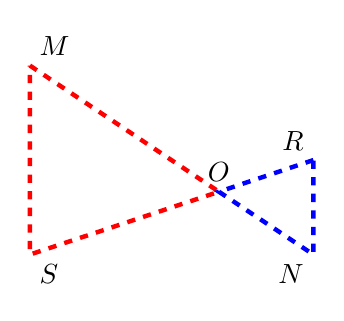
\begin{tikzpicture}[scale = 0.6]
            % \draw[help lines, color=black!30, dashed] (0,0) grid (10,7);        
            \coordinate[label=above right:$M$] (M) at (1,5);
            \coordinate[label=below left:$N$] (N) at (7,1);
            \coordinate[label=below right:$S$] (S) at (1,1);
            \coordinate[label=above left:$R$] (R) at (7,3);
            \coordinate[label=above:$O$] (O) at (5,2.33);
            \tkzDrawLine (M,N);
            \tkzDrawLine (S,R);
            \tkzDrawLine (M,S);
            \tkzDrawLine (R,N);
            \draw[dashed, color=red, ultra thick](M)--(O)--(S)--(M);
            \draw[dashed, color=blue, ultra thick](R)--(O)--(N)--(R);
        \end{tikzpicture}
    \end{minipage}
    \begin{multicols}2
        \begin{enumerate}
            \item Le tableau \ding{193} est un tableau de proportionnalité.

            \begin{tabular}{c|c|c}
                $\textcolor{blue}{NO}$&$\textcolor{blue}{RO}$&$\textcolor{blue}{RN}$\\ \hline
                $\textcolor{red}{OM}$&$\textcolor{red}{OS}$&$\textcolor{red}{MS}$\\
            \end{tabular}

            \item Pour le tableau \ding{192}, la première colonne n'est pas proportionnelle aux deux autres.
            $RS$ n'est un côté d'aucun des deux triangles.Il aurait fallu avoir $OR$ à la place de $RS$.

            \begin{tabular}{c|c|c}
                $\textcolor{red}{OS}$&$\textcolor{red}{OM}$&$\textcolor{red}{MS}$\\ \hline
                $\textcolor{black}{RS}$&$\textcolor{blue}{ON}$&$\textcolor{blue}{RN}$\\                 
            \end{tabular}
            \columnbreak
            
            Pour le tableau \ding{194}, la deuxième colonne n'est pas proportionnelle aux deux autres.
            Il y a un souci au niveau des côtés des triangles. Il aurait fallu inverser $ON$ et $OM$.

            \begin{tabular}{c|c|c}
                $\textcolor{red}{OS}$&$\textcolor{blue}{ON}$&$\textcolor{red}{MS}$\\ \hline
                $\textcolor{blue}{OR}$&$\textcolor{red}{OM}$&$\textcolor{blue}{RN}$\\                 
            \end{tabular}
        \end{enumerate}
    \end{multicols}
\end{corrige}

